\subsection{Transit Fits}

After the transit searches were performed for OBS, INJ, INV and SCR, we discovered that the transit fit portion of DV had an error that caused the impact parameter for each fit to be biased towards large values, causing the planet radii to be too large. See \citet{KSCI19110}. Since a consistent set of reliable transit fits are required for all TCEs, we created the supplemental transit fits.  The same DV transit fitting code was given as an initial condition for the fit, the KIC, period, epoch and MES of the original detection. These supplemental fits do not have the same impact parameter bias of the original. See Figure~\ref{f:dvfits} for the distribution of the impact parameters and planet radii for both the original and the supplemental DV fits.  Sometimes the DV fitter fails to converge and in these cases we were not able to obtain a supplemental transit fit. Also, at times the epoch wanders too far from the original detection; in these cases we do not consider it to be a successful fit since we intend to fit the same signal as that detected by TPS.

As a result, this catalog depends on four different transit fits: 1) the original DV transit fits, 2) the trapezoidal fits performed on the alternate detrending light curves, 3) the supplemental DV transit fits and 4) the MCMC fits (\S\ref{s:mcmc}.  Because the bug in the transit fits was only discovered after all of the metrics for the Robovetter were run, the original and trapezoidal fits were used to disposition the TCEs.  The supplemental fits are used to understand the completeness and reliability of the catalog as a function of fitted parameters (such as planet radii or insolation flux).  The MCMC fits are only provided for the KOI population. In a statistical sense the MCMC fits are consistent with the supplemental fits. %\citet{ChristiansenKSCI} demonstrates how the planet radii of the injected planets measured by the supplemental and the MCMC fits agree. 
For the planet candidates in DR25 we plot the planet radii of the MCMC fits against the supplemental fits; see Figure~\ref{f:mcmcsupp}. While some individual systems may disagree by quite a bit, from a statistical sense, the two populations agree well within the errors. 

\begin{figure}
\centering
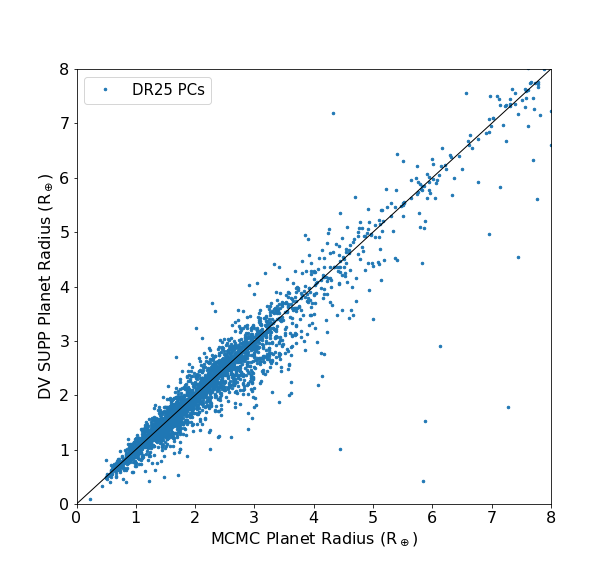
\includegraphics[width=0.99\linewidth]{fig-comparePradius-mcmcSup.png}
\caption{Comparison of the DR25 PCs fitted planet radii measured by the MCMC fits and the DV supplemental fits. The 1:1 line is drawn in black. While individual objects have different fitted values, statistically the planet radii from the two fits agree. }
\label{f:mcmcsupp}
\end{figure}


[SOMEONE needs to make this section more ROBUST. Is the planet radii all we need to consider?]
